% !TEX root =  master.tex 
%Hauptteil!
\chapter{Erstes Konzept -- Daniel Pies}

\section{Use-Case}

Um ein erstes Grundkonzept eines Bauunternehmens zu haben, haben wir uns überlegt, was braucht unser Unternehmen unbedingt. Dabei sind uns einige Attribute wie ein Kontostand, Mitarbeiter, Material und einige Maschinen zuerst eingefallen. Diese Maschinen und das Material muss der Spieler anschaffen können. Außerdem muss er die Mitarbeiter einstellen können.

Des Weiteren haben wir überlegt, wir brauchen vorerst nur zwei Spieler, die jeweils ihr eigenes Unternehmen haben, dann beide ihre Spielzüge durchführen können und dann die Berechnung der aktuellen Spielrunde starten können. Nach einer beliebigen Runde sollen die Spieler das Spiel beenden können und ein Gewinner muss vom Spiel ermittelt werden. Daraus ist folgendes Use-Case Diagramm entstanden:

\begin{minipage}{\linewidth}
	\centering
	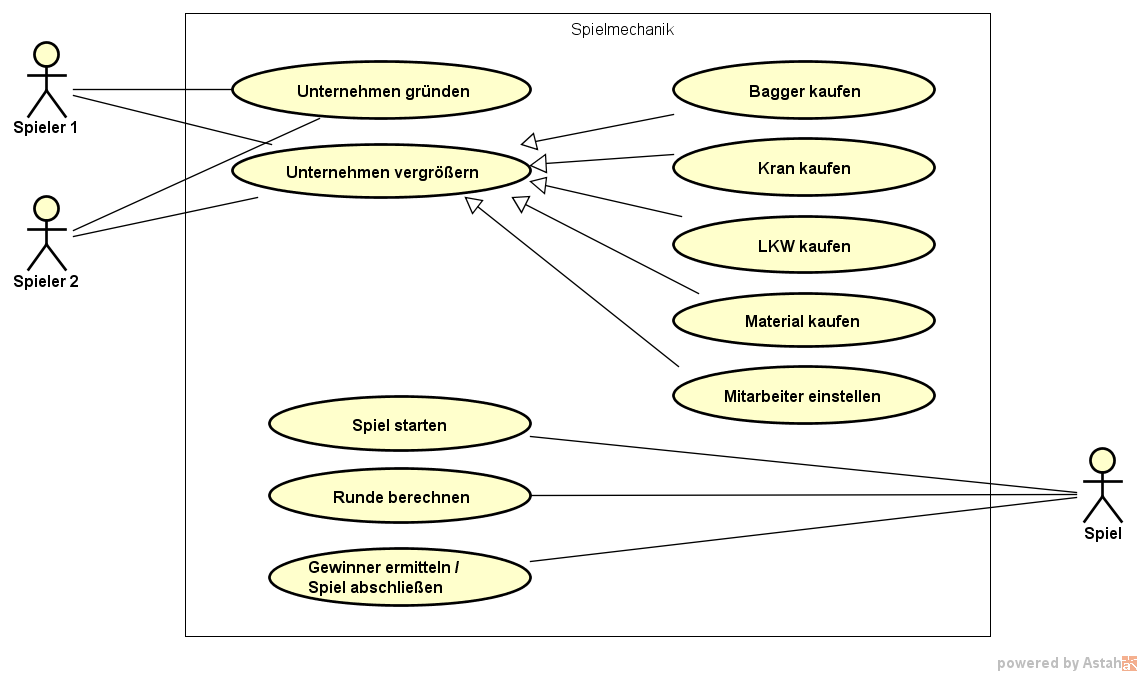
\includegraphics[scale=0.4]{img/UseCasePrototypeFallstudie.png}
	\captionof{figure}{\label{abb:usecase1}Use-Case Diagramm des ersten Prototypen}
	\vspace{2em}
\end{minipage}

\section{Klasssendiagramm}

Aus diesem Use-Case Diagramm ist dann folgendes Klassendiagramm entstanden:

\begin{minipage}{\linewidth}
	\centering
	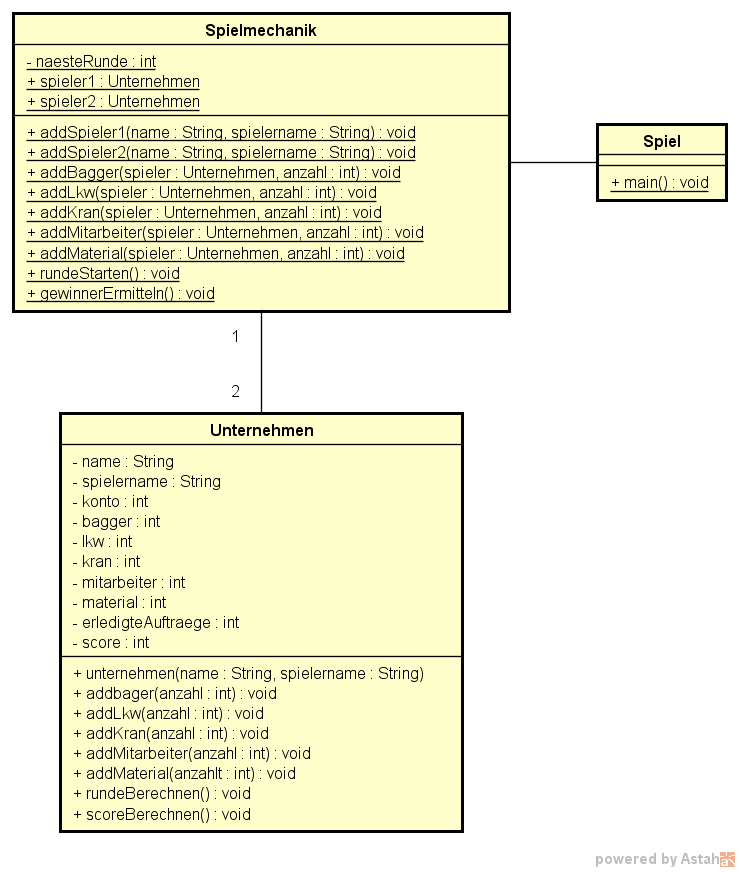
\includegraphics[scale=0.63]{img/ClassDiagramPrototypeFallstudie.png}
	\captionof{figure}{\label{abb:classdiag1}Klassendiagramm des ersten Prototypen}
	\vspace{2em}
\end{minipage}

Bei dieser Programmierung stellt die Klasse \glqq Unternehmen\grqq \ den Spieler samt seines Unternehmens dar. Die Klasse \glqq Spielmechanik\grqq \ erzeugt zum Spielstart die beiden Spieler, also zwei Instanzen der Klasse \glqq Unternehmen\grqq . Über die Klasse \glqq Spiel\grqq \ erfolgen die Eingaben an das Spiel. In ihr befindet sich auch die Main-Methode, die zum Spielstart ausgeführt werden muss. 

\section{Spiel Beispiel}

Ein mögliches Spiel wie es in der Klasse \glqq Spiel\grqq \ gespielt werden könnte, sieht zum Beispiel so aus:

\lstset{language=Java}
\begin{lstlisting}[caption={Beispiel für die Klasse \glqq Spiel\grqq}, label={lst:prototypspiel}]
public class spiel {

public static void main(String[] args) {

spielmechanik.addSpieler1("ABC Bau GmbH", "Daniel Pies");
spielmechanik.addSpieler2("XYZ Bau OHG", "Manuel Techert");

spielmechanik.addBagger(spielmechanik.spieler1, 2);
spielmechanik.addKran(spielmechanik.spieler1, 1);
spielmechanik.addLkw(spielmechanik.spieler1, 1);
spielmechanik.addMitarbeiter(spielmechanik.spieler1, 3);

spielmechanik.addBagger(spielmechanik.spieler2, 1);
spielmechanik.addKran(spielmechanik.spieler2, 1);
spielmechanik.addLkw(spielmechanik.spieler2, 2);
spielmechanik.addMaterial(spielmechanik.spieler2, 10);

spielmechanik.rundeStarten();

spielmechanik.addBagger(spielmechanik.spieler1, 2);
spielmechanik.addMitarbeiter(spielmechanik.spieler1, 5);

spielmechanik.addLkw(spielmechanik.spieler2, 2);
spielmechanik.addMaterial(spielmechanik.spieler2, 10);

spielmechanik.rundeStarten();

spielmechanik.gewinnerErmitteln();

}

}

\end{lstlisting}